\documentclass[UTF8,adobefonts]{ctexart}
\usepackage[top=2cm,left=2cm,right=2cm,foot=1.5cm,bottom=2cm]{geometry}
\usepackage[colorlinks,linkcolor=red,anchorcolor=blue,citecolor=green]{hyperref}
\usepackage{graphicx}
\usepackage{amsmath}
\usepackage{textcomp}
\usepackage{vector}
\begin{document}
\title{Octave入门}
\author{\it 莫及\footnote{liuqiang@coer.zju.edu.cn}}
\date{2011年1月}
\maketitle
\tableofcontents
\newpage
\section{简介}
\subsection{Octave是什么?}
Octave是一款用于数值计算和绘图的开源软件。和Matlab一样,Octave尤其精于矩阵运算:求解联立方程组、计算矩阵特征值和特征向量等等。
在许多的工程实际问题中,数据都可以用矩阵或向量表示出来而问题转化为对这类矩阵的求解。另外,Octave能够通过多种形式将数据可视化,
并且Octave本身也是一门编程语言而易于扩展。因此我们可以称Octave是一款非常强大的可编程可视化计算程序。Octave让解决很大范围内的
数值问题变得简单,给使用者更多的时间来进行实验和考虑问题。

Octave最初被开发时只是一款用于本科生化学课程的辅助程序。当前Octave项目的开发由J.W.Eation博士领导
并遵循GNU General Public Licence发布。Octave与科研和工程中普遍使用的Matlab基本兼容,因此其易用性也越来越好。
\subsection{Octave不是什么?}
Octave是用于数值地解决数学问题的,即在计算机内存内处理相应的数值。因此Octave和Mathematica、Maple这类通过数学推导给出问题符号解
的程序不同,它不能给出问题的精确解。这无所谓好或者坏——不同软件处理不同的问题罢了。而且,很多实际的数学问题(尤其是工程问题)都没有解析解。
\subsection{Octave的适用对象}
Octave和Maltab被工程人员和科研人员广泛使用来进行各种工业和学术上的数值计算和仿真。例如,NASA使用它来开发飞行器的对接系统;
Jaguar Racing使用它来可视化和分析从F1赛车传来的数据;Sheffield 大学用它来开发用于识别癌细胞的软件。Octave这样的
软件让编写数值处理程序变得简单,并提供数据可视化的多种方式。
\subsection{与常见的高级语言(如C++)的区别}
C++以及其他的常用的编程语言更多得用来编写具有特定功能的软件。然而,使用C++来处理数值方面的问题过于复杂费时,
而且这样的编程语言不原生的支持一些数学概念或者生成图形。Octave是专为解决这类问题而设计的。即使人们最终使
用C++这样的语言来编写软件,他们很多时候都用Octave来编写软件的原型或者数学部分,因为这样能够很快的检验其算法。
\section{简单计算}
\subsection{启动Octave}
Octave在UNIX环境下通过在终端中输入octave来启动,在启动octave之后,程序一般会显现如下这样的信息:
\begin{verbatim}
GNU Octave, version 3.2.4
Copyright (C) 2009 John W. Eaton and others.
This is free software; see the source code for copying conditions.
There is ABSOLUTELY NO WARRANTY; not even for MERCHANTABILITY or
FITNESS FOR A PARTICULAR PURPOSE.  For details, type `warranty'.

Octave was configured for "i486-pc-linux-gnu".

Additional information about Octave is available at http://www.octave.org.

Please contribute if you find this software useful.
For more information, visit http://www.octave.org/help-wanted.html

Report bugs to <bug@octave.org> (but first, please read
http://www.octave.org/bugs.html to learn how to write a helpful report).

For information about changes from previous versions, type `news'.
Octave:1>
\end{verbatim}
这表明你已经进入了Octave环境,其中 {\tt Octave:>1}为Octave命令提示符。

如果你要退出Octave,只需要在命令提示符下输入quit或者exit即可。
\subsection{Octave简单计算}
\begin{table}[htbp]
\caption{基本数学函数}
\label{tb:basicfunc}
\centering
\begin{tabular}{p{100pt}p{200pt}}
\hline
cos 	& 余弦函数(弧度制) \\
sin 	& 正弦函数(弧度制) \\
tan 	& 正切函数(弧度制) \\
exp 	& 指数函数($e^x$)\\
log 	& 以e为底的指数函数 \\
log10 	& 以10为底的指数函数 \\
sinh 	& 双曲正弦函数 \\
tanh 	& 双曲正切函数 \\
cosh 	& 双曲余弦函数 \\
acos 	& 反余弦函数 \\
acosh 	& 反双曲余弦函数 \\
asin	& 反正弦函数 \\
asinh	& 反双曲正弦函数 \\
atan	& 反正切函数 \\
atan2	& 双参数形式的反正切函数\footnote{atan2(Y,X)=atan(Y/X)} \\
atanh	& 反双曲正切函数 \\
\hline
abs	& 绝对值函数(复数取模) \\
sign	& 符号函数 \\
round	& 四舍五入\\
floor	& 近似为比它小的最大整数 \\
ceil	& 近似为比它大的最小整数 \\
fix	& 向0方向近似 \\
rem	& 求余数 \\
\hline
\end{tabular}
\end{table}
Octave最简单的使用方式就是像使用一个计算器一样在命令提示符下输入相应的计算式。Octave能识别通常的计算表达式。
例如,在终端输入
\begin{verbatim}
octave:##>2+2 
\end{verbatim}
并按回车键,你将得到以下的结果
\begin{verbatim}
  ans=4
\end{verbatim}
各种计算符号的优先级与常规的一致,比如括号有最大优先级,其次为乘方,其次为乘除运算,最后为加减运算。
\subsection{内建函数}
除了一些基本的计算符,Octave还提供了一系列的常用数学函数,其中的一部分函数如表~\ref{tb:basicfunc}~所示。
像C++中调用函数一样,Octave通过输入函数名和括号中的输入参数来调用函数,例如:
\begin{verbatim}
 octave:##> exp(1)
    ans=2.71813
\end{verbatim}
又如另一个更长的表达式:计算$1.2\sin(40^\circ+\ln(2.4^2))$,输入
\begin{verbatim}
 octave:##>1.2*sin(40*pi/180+log(2.4^2))
    ans=0.76618
\end{verbatim}
在刚才的例子中,有以下的注意事项:
\begin{enumerate}
\item 在计算表达式中一个明确的乘号是必不可少的,比如在1.2和sin之间必须要的乘号。
\item 三角函数是使用的弧度制。角度制的可以通过乘以引子$\pi/180$转换为弧度制。
pi是Octave中变量的一个例子,这将在下一节中详细介绍。
\item 自然对数是用‘log’ 而不是 ‘ln’ 来表示的。
\end{enumerate}
通过使用这些函数,Octave能完成你用普通计算器来完成的所有计算。

\section{Octave环境}
从之前的几个例子可以看出,Octave有一个命令行界面——每个命令依次输入命令行中,并以回车
结束。Octave为解释性语言,即每个命令通过命令解析器转化为机器语言。而在编译型语言,如C++
中,整个程序通过文本编辑器输入并通过编译器将整个代码转化为机器语言。这样的编译型语言比
解析型语言运行速度快很多。然而由于Octave这样的语言能很快的将代码实现,这样弥补了其运行
速度方面的缺陷。
\subsection{变量}
在实际的计算中,你都需要存储并再利用一些数值,正如计算器中的存储器一样。Octave允许你
定义并使用变量。例如,在之前的角度问题中,我们可以定义一个名为{\tt deg}的变量来保存
角度与弧度换算的因子:
\begin{verbatim}
 octave:##> deg=pi/180
    deg=0.017453
\end{verbatim}

注意和很多的高级语言(如C++)不同,Octave中变量的类型是不用声明的。Octave所有的变量都是
浮点型或者字符串。运用这个变量,之前的表达式可以重写为:
\begin{verbatim}
 octave:##>1.2*sin(40*deg+log(2.4^2))
    ans=0.76618
\end{verbatim}

这能使表达式更容易输入和易懂,避免因为粗心大意引起的一些低级错误等。在写程序的时候,请尽量
将你的一些常用数字和结果用变量表示。

你已经见到过的另一个Octave变量便是{\tt ans}变量。这个变量存储你每次最近运算的结果。这个变量
同样可以像普通变量一样供我们使用。例如:
\begin{verbatim}
 octave:##> new=3*ans
    new=2.2985
\end{verbatim}
注意new的数值也不是单单计算$3\times0.76618$得到的结果。这是因为Octave的结果只以一定的精度
展示出来,而实际上它存储的变量的精度要比其显示的高很多,因此实际的结果要比2.2985精确很多。在
所有的数值计算中,数值的有效位数是很重要的因素。因此使用变量名而不是每次输入结果能够尽量的
避免数值的截断误差。

在定义和使用变量时,Octave中变量名是区分大小的,即变量a和变量A是不同的变量。而且Octave本身
已经定义了一些变量,如 pi,i和j($i=j=\sqrt{-1}$(见第十四节))等。Octave不会阻止你重新
定义这些内置变量,但是这样的操作会让你的程序变得含糊。同样的,类似于{\tt sin}和{\tt cos}
这样的变量也是允许的,但不提倡。

如果你需要查看某个变量的数值,输入其变量名并回车即可。如果你想查看当前名命名或者使用的
函数名和变量名,输入
\begin{verbatim}
octave:##> who
*** dynamically linked functions:
dispatch
*** currently compiled functions:
rem
*** local user variables:
deg new
\end{verbatim}

如果你需要从当前的变量空间中删除某个变量,{\tt clear}命令能移出所有的变量,或者移出某个
特定变量,如:
\begin{verbatim}
 clear name
\end{verbatim}
将移出名为{\tt name}的某个变量。
\subsection{数值及其格式}
我们发现Octave通常只显示一定的有效数字。{\tt format}命令能让你选择数值显示的不同方式。
输入
\begin{verbatim}
 octave:##> format long
\end{verbatim}
将让octave以15位的有效数字显示数值,这也是octave程序本身的计算精度。输入$\tt help format$
你将得到本命令的所有选项的列表。通过使用{\tt format long}命令,我们将看到更加精确的{\tt deg}
数值:
\begin{verbatim}
 octave:##> deg
    deg=0.0174532925199433
 octave:##> format short
\end{verbatim}
其中第二行将让octave以默认的方式显示数值。

Octave使用科学记数法来表达数值很大或者很小的数字,例如 $13142.6=1.31426\times10^4$,而
在Octave中这个科学数值被显示为{\tt 1.3143e+04},这样的数值输入形式也同样能被Octave认可。

同样被Octave识别并计算的数据形式还有:
\begin{description}
 \item {\emph{复数}} (e.g.{\tt 3+4i}),能完全被Octave识别,具体的内容将在第十四节中讲述。
 \item {\emph{无穷大}} (Inf) 一个数除以0得到的结果。
 \item {\emph{非数值}} (NaN) 0除以0得到的结果。同样是其他数学表达式无法得到合法结果时的返回值。
\end{description}
Inf和NaN可以向其他类型的数据一样参与运算,当然得到的结果通常还是Inf或者NaN。
\subsection{数值的表示和精度}
Octave中的数值,通计算机中存储的数值一样,是用二进制的形式而不是十进制的形式存储的。在十进制
的数值表达中,12.25的意义是
\begin{equation}
 12.25=1\times10^1+2\times10^0+2\times10^{-1}+5\times10^{-2}
\end{equation}
但是在二进制的表达中,这将被写为
\begin{equation}
 1101.01=1\times2^3+1\times2^2+0\times2^1+1\times2^0+0\times2^{-1}+
1\times2^{-2}=12.25
\end{equation}
二进制形式的数值适合电脑存储是因为这样的数据只是一系列的0或者1,对应于电路中的开和关的状态。
用二进制表示数据的一个问题是在电脑中每个数值只能以有限的位数(bit)来表示,即其位数为有限值。
考虑如下的例子:
\begin{verbatim}
 octave:##> 1-0.2-0.2-0.2-0.2-0.2
    ans=5.5511e-17
\end{verbatim}
得到了一个非常小的结果,但是不是零这个精确的解。造成这样的问题的原因在于在计算机中0.2
无法使用有限的位数的二进制精确表示出来(0.2=0.0011001100...)。这样的情况与在十进制中
1/3无法精确写出的原因是一致的。在Octave(和其他计算机程序中),这样的数值以最能接近精确值的
方式存储和运用起来。但是,如同在这里看到的这般,这样的近似是容易引起问题的。基于这样的原因,
在考虑两个数值是否相等的时候,不要忘了其精度和容许误差。
\subsection{载入和保存数据}
当你退出Octave的时候,你将丢失你所创建的变量。如果你需要在工作的中途退出Octave,那么你可以
保存当前会话的数据并在之后重新载入它。如果你输入
\begin{verbatim}
 octave:##> save anyname
\end{verbatim}
这将整个工作空间上的变量存储到当前目录下一个名为{\tt anyname.mat}的文件中(注意{\tt .mat}
是octave自动添加的)。这样你可以退出Octave,之后重新启动Octave程序,通过输入
\begin{verbatim}
 octave:##> load anyname
\end{verbatim}
将重新载入之前保存的命名空间,并从你中断的地方重新开始工作。同样的,你可以载入或者保存特定的变量。
格式为
\begin{verbatim}
 octave:##>save filename var1 var2 ...
\end{verbatim}
例如,如果你想存储{\tt deg}变量,那么你可以输入
\begin{verbatim}
 octave:##> save degconv deg
\end{verbatim}
这样将{\tt deg}变量存储于名为{\tt degconv.mat}的文件中,你可以通过以下命令重新载入变量
\begin{verbatim}
 octave:##> load degconv
\end{verbatim}
Octave 同样能从文件中导入数据,这样的功能在你使用其他的数据来源进行画图或者计算的时候变得非常
有用。
\subsection{重复之前命令}
Octave会记录你在一个会话中输入过的命令,而你可以通过方向键中的 $\downarrow$ 和 $\uparrow$ 来查看
之前输入的命令(最近的命令排列在最前)。如果你想重复其中的一个命令,你只需要用方向键找到
该命令并按回车。

一旦一个已执行命令被重新调出来,你可以在再次执行它之前编辑它。你可以用$\leftarrow$ 和 $\rightarrow$
移动光标并进行相应的编辑操作。当你输入一个长的Octave命令并出错的时候,这样的功能便会很有帮助。
\subsection{获得帮助}
如果你不了解某个Octave命令的功能或者是你需要找一个特定的函数,Octave本身强大的帮助
系统会很有用。最基本的使用帮助系统的方式就是
\begin{verbatim}
 help commandname
\end{verbatim}
例如:
\begin{verbatim}
 octave:1> help sqrt
 `sqrt' is a built-in function

 -- Mapping Function:  sqrt (X)
     Compute the square root of each element of X.  If X is negative, a
     complex result is returned.  To compute the matrix square root, see
     *note Linear Algebra::.

     See also: realsqrt



Additional help for built-in functions and operators is
available in the on-line version of the manual.  Use the command
`doc <topic>' to search the manual index.

Help and information about Octave is also available on the WWW
at http://www.octave.org and via the help@octave.org
mailing list.

\end{verbatim}
如果你不知道你需要的某个函数的具体名称,有几个方法可以帮助你找到这样的函数是否存在。
通过命令行输入{\tt help -i},Octave将给出一个其帮助的主题列表。

关于某个帮助主题的细节可以通过将光标移动到该主题并回车获得。 你可以通过{\bf U}p,{\bf N}ext,
{\bf Previous} 等快捷键浏览相应的主题。或者在命令提示符下直接输入话题的名称如arithmetic
方面的帮助可以输入
\begin{verbatim}
 octave:##> help -i arithmetic
\end{verbatim}
来获得。输入‘{\bf q}’来退出帮助系统并返回到octave命令行。
\subsection{取消一个命令}
如果你发现输入的一个命令执行了很长的时间(或者你程序本身的bug让程序无限重复等),中止该程序
的执行就变得又必要。你可以在当前命令行下输入
\begin{verbatim}
 Ctrl-C
\end{verbatim}
程序将被中止并返回到命令提示界面。
\subsection{分号和隐藏结果}
分号在通常的编程语言中被用来表示程序块或者单个语句的结束。在Octave中分号不是必需的,但
它也有一个特殊的功能。我们目前的例子中,我们只要输入一个Octave命令并不以分号结尾的话,
Octave总会将语句执行的结果随即显示出来。但是,如果我们在一行语句的末尾添上分号,Octave将
不会显出相应的结果。
%section 4
\section{数组和向量}
在很多的数学问题中涉及到一组数据。在编程语言中这样的数据通常被称为数组(array)。在Octave中
这样的概念被称为向量(vector),而向量本身也是矩阵类数据的一个特例——只有一行或者一列的矩阵分别
为行向量($\cdots$)或者列向量($\vdots$)。

\subsection{构造向量}
构造矩阵或者向量的方法有很多。其中最直接简单的方法就是在一个方括号[]中给出其元素,例如
\begin{verbatim}
 octave:##> a=[1 4 5]
    a=
      1 4 5
 octave:##> b=[2,1,0]
    b=
      2 1 0
 octave:##> c=[4;7;10]
    c=
      4
      7
      10

\end{verbatim}
在方括号中由空格或者逗号隔开的一组数据被定义为行向量;而由分号或者回车隔开的一组数据被定义为
列向量。

你可以通过已经定义的向量来定义新的向量,例如
\begin{verbatim}
 octave:##> a=[1 4 5]
    a=
      1 4 5
 octave:##> d=[a 6]
    d=
      1 4 5 6
\end{verbatim}

\subsection{冒号表达式}
利用冒号能够非常方便的创建一些特殊的向量
\begin{verbatim}
 octave:##> e=2:6
    e=
      2 3 4 5 6
\end{verbatim}

冒号表达式的规则是告诉octave创建一个以第一个数字开始并以一递增至第二个数的向量。在第一和
第二个数之间可以插入第三个参数来声明向量中元素之间的递增量,形如$a:b:c$。
\begin{verbatim}
 octave:##> e=2:0.3:4
    e=
      2.0000 2.3000 2.6000 2.9000 3.2000 3.5000 3.8000
\end{verbatim}
如这个例子所示,如果向量中的增量不是恰好达到尾数,octave将产生不超过尾数的一组向量。增量可以
是负数并相应产生有一个递减的向量。

\subsection{大矩阵或矩阵的显示}
如果Octave无法用单屏显示一个向量或者矩阵,它将分屏显示这个量比如
\begin{verbatim}
 octave:##> v=1:1000
\end{verbatim}
按空格键来显示下一屏的内容而按'q'退出显示并返回到Octave命令提示符。你同样可以按‘b’键
向上翻页并查看已显示的内容。

如果你想关闭Octave的这个显示功能,输入
\begin{verbatim}
 octave:##> more off
\end{verbatim}
命令即可。这个功能通过以下命令可以重新打开
\begin{verbatim}
 octave:##> more on
\end{verbatim}
\subsection{向量构造函数}
Octave提供更多的创建向量的函数,如表~\ref{tb:vectorfun}~所示。
\begin{table}[htbp]
\caption{基本数学函数}
\label{tb:vectorfun}
\centering
\begin{tabular}{|p{100pt}p{200pt}|}
\hline
zeros(M,N)	& 创建一个M$\times$N的零矩阵\\
ones(M,N)	& 创建一个M$\times$N的全译矩阵\\
linspace(x1,x2,N)	& 创建一个N个元素的向量,均匀分布于x1和x2\\
logspace(x1,x2,N)	& 创建一个N个元素的向量,指数分布与$10^{x1}$和$10^{x2}$之间\\
\hline
\end{tabular}
\end{table}

其中{\tt zeros}和{\tt ones}适用于向量和矩阵,而这两个函数的参数,M和N,分别指定矩阵的
行数和列数。有关矩阵的内容将在第九节中讲解。
\subsection{向量中的元素操作}
向量中的元素通过括号$()$,而第一个元素的编号为1,而不是像C或者C++那样从0开始。例如
\begin{verbatim}
 octave:##> a=[1:2:6 -1 0]
    a=
      1 3 5 -1 0
\end{verbatim}
我们可以通过以下命令访问到该向量的第三个元素
\begin{verbatim}
 octave:##> a(3)
    ans=
      5
\end{verbatim}
冒号的表示法同样可以用于声明向量中的元素的范围
\begin{verbatim}
 octave:##> a(3:5)
    ans=
      5 -1 0
 octave:##> a(1:2:5)
    ans=
      1 5 0
\end{verbatim}
\subsection{向量的计算}
将一组数据存入一个向量之后能够使用很多的Octave函数来进行计算。在C++中如果你想进行相同的
计算,例如每个元素乘以2,你需要使用for循环来对每个元素操作。在Octave中虽然也可以使用for
循环来实现,但是Octave本身由有简单的向量操作方式。

向量中每个都乘以一个数可以通过对该向量乘以一个数来实现。以之前定义的{\tt a}向量为例:
\begin{verbatim}
 octave:1> a=[1:2:6 -1 0]
a =

   1   3   5  -1   0

 octave:2> a*2
ans =

    2    6   10   -2    0

\end{verbatim}
对向量中所有元素都除以一个数的操作与乘法类似。使用$+-$算符,你同样可以对该向量中的每个元素都
加上或者减去一个数值。

两个向量的相乘遵循矩阵的乘法法则,向量乘法并不是对应元素的相乘。如果要进行对应元素的
乘除法,你可以使用\begin{verb}.* ./\end{verb}算符,例如
\begin{equation}
\begin{pmatrix}a_1\\a_2\\a_3\end{pmatrix}.* \begin{pmatrix}b_1\\b_2\\b_3\end{pmatrix}
=\begin{pmatrix}a_1b_1\\a_2b_2\\a_3b_3\end{pmatrix}
\end{equation}
注意每个算符前的‘$\ldotp$’表示为一个元素对元素的计算。例如:
\begin{verbatim}
 octave:3> b=1:5
b =

   1   2   3   4   5

 octave:4> a.*b
ans =

    1    6   15   -4    0

\end{verbatim}
逐个元素的乘方计算同样也很有用。该计算的算符为,例如
\begin{verbatim}
 octave:5> b.^2
ans =

    1    4    9   16   25

 octave:6> 2.^b
ans =

    2    4    8   16   32
 octave:7> a.^b
ans =

     1     9   125     1     0
\end{verbatim}
只要两个向量又相同的大小和形状,它们就可以进行元素之间的(element-by-element)加减乘除和乘方运算。
大多数的Octave函数能以向量为输入。例如,创建一个以60度为间隔的角度值,并作为{\tt sin}
函数的输入:
\begin{verbatim}
 octave:8> angles=[0:pi/3:2*pi]
angles =

   0.00000   1.04720   2.09440   3.14159   4.18879   5.23599   6.28319

octave:9> y=sin(angles)
y =

   0.00000   0.86603   0.86603   0.00000  -0.86603  -0.86603  -0.00000

\end{verbatim}

%section 5
\section{画图}
\begin{figure}[htbp]
\centering
\includegraphics[width=0.6\textwidth]{sinx.eps}
\caption{$y=\sin(x)$图形,60度间隔}
\label{sin1}
\end{figure}
Octave通过调用另一个开源软件GNUPLOT\footnote{www.gnuplot.org}来实现非常
丰富的画图功能\footnote{若是对图片的细节要求更高,推荐将数据格式化输出并单独使用
gnuplot生成图形}。最基本的画图命令是{\tt plot(x,y)},其中{\tt x,y}分别为
横轴和纵轴数据。上一节生成的正弦函数的图形可以通过以下命令获得
\begin{verbatim}
 octave:10> plot(angles,y)
\end{verbatim}
程序会打开一个新的窗口显示该图片,如图~\ref{sin1}~所示。Octave会根据图形属性
中自动选择坐标范围。

该图形过于粗糙,使用更精细的{\tt y}值能获得更加精确的图片。
\begin{verbatim}
 octave:1> angles=linspace(0,2*pi,100);
 octave:2> y=sin(angles);
 octave:3> plot(angles,y);
\end{verbatim}
其中{\tt linspace}命令创建了0到$2\pi$之间的100个数值。
\subsection{改进该图形}
在Octave中你可以在{\tt plot}命令中加入更多的选项拉指定图形线条的样式。例如,
使用红色和圆圈来画出之前的图片,输入
\begin{verbatim}
 octave:4> plot(angles,y,'ro');
\end{verbatim}
其中最后一个参数是指定线条样式的字符串。表~\ref{tab:style}~列出所有
可能的选项(同样可以使用{\tt help plot}获得)。
\begin{table}
\centering
\caption{{\tt plot}命令中的颜色和样式选项(见{\tt help plot}),($\dag$仅在Matlab中存在的选项)}
\label{tab:style}
 \begin{tabular}{|l|l|l|}
  \hline
 w 白色 & . 点 & - 实线 \\
 m 品红 & o 圆圈 & : 虚线$\dag$ \\
 c 青色 & x x形 & -. 点划线$\dag$ \\
 r 红色 & + +号 & -- 虚线$\dag$ \\
 g 绿色 & * 星号 & \\
 b 蓝色 & s 正方形 $\dag$& \\
 y 黄色$\dag$ & d 菱形$\dag$ & \\
 k 黑色$\dag$& v 下三角$\dag$ & \\
 %& \^{} 上三角 & \\
 & < 左三角$\dag$ & \\
 & > 右三角$\dag$ & \\
 & p 五角星$\dag$ & \\
 & h 六边形$\dag$ & \\
\hline
 \end{tabular}
\end{table}
通过{\tt title},{\tt xlabel}和{\tt ylabel}命名为该图片添加标题和xy轴名称:
\begin{verbatim}
 octave:7> title('Graph of y=sin(x)')
 octave:8> xlabel('Angle')
 octave:9> ylabel('Value')
\end{verbatim}
使用{\tt replot}命令来更新图片。{\tt grid}命令为图片添加网格线:
\begin{verbatim}
 octave:##> grid on
\end{verbatim}
图~\ref{improvedsinx}~显示了最新的结果。
\begin{figure}
 \centering
 \includegraphics[width=0.6\textwidth]{improvedsinx.eps}
 \caption{每个点使用红色圆圈的$y=\sin(x)曲线$}
  \label{improvedsinx}
\end{figure}
\subsection{Multiple graphs}
一幅图上可以画多条曲线。通过在{\tt plot}命令中按照次序给出每条曲线的{\tt x}和{\tt y}
向量。例如,在之前的正弦曲线的基础之上画出余弦曲线:
\begin{verbatim}
 octave:##>plot(angles,ycangles,cos(angles));
 octave:##>legend('Sine','Cosine');
\end{verbatim}
而{\tt legend}命令为该图片添加相应的图例。该图片的结果如图~\ref{sinandcos}~所示。
到目前为止,用户在新输入{\tt plot}命令之后,原图片上的内容将被删除。如果你想
保存当前的图片内容并将新创建的图片层叠到原图片上,你可以通过使用{\tt hold}命令
来实现。使用该命令,我们可以实现在同一幅图上呈现由两个{\tt plot}命令绘制的线条。
\begin{verbatim}
 octave:13> plot(angles,y,'.')
 octave:14> hold on
 octave:15> plot(angles,cos(angles),'g-')
 octave:16> legend('Sine','Cosine')
\end{verbatim}
而命令{\tt hold off}将会关闭该功能。
\begin{figure}
 \centering
 \includegraphics[width=0.6\textwidth]{sinandcos.eps}
 \caption{$y=\sin(x)$和$y=\cos (x)$曲线}
 \label{sinandcos}
\end{figure}
\subsection{Multiple figures}
 多幅图片可以通过{\tt figure}命令来控制。在命令行中输入
\begin{verbatim}
 octave:##> figure
\end{verbatim}
那么下一个{\tt plot}命令将会在新创建的窗口中绘制。例如
\begin{verbatim}
 octave:##> plot(angles,tan(angles))
\end{verbatim}
将会在该新窗口中画出正切函数图像。如果你想返回到之前的图片,输入
\begin{verbatim}
 octave:##> figure(1)
\end{verbatim}
即可。
\subsection{保存和打印图片}
Octave/Gnuplot没有提供鼠标或者快捷键操作来实现图片的打印操作。然而Octave提供了print命令
来将图片打印到默认的打印机上。{\tt help print}命令给出所有的{\tt print}命令提供的选项,包括
\begin{verbatim}
 octave:##> print('graph1.eps','-deps')
\end{verbatim}
来保存当前图像到一个eps文件或者
\begin{verbatim}
 octave:##> print('graph1.png','-dpng')
\end{verbatim}
将当前图像保存为一个png文件。
%section 6
\section{Octave编程I:脚本文件}
如果你有一些重复输入的命令的,你可以将这一系列的命令存入一个Octave脚本之中。这种包含Octave命令
的文本文件是Octave程序的基本形式。当你在Octave中执行这样的脚本的时候,其效果与将这些命令一行行
输入Octave中的效果是一样的。而且当你对一系列要输入Octave的命令不是很拿的准的时候,在一个脚本中
修改这些命令会比在Octave终端中重新调出及修改命令要简单方便许多。

Octave的脚本是普通的文本文件, 但是他们需要有一个{\tt .m}的后缀(e.g. run.m)。因此,它们通常
也被称为M文件。除去后缀的文件名部分是你在执行该命令时需要向Octave终端输入的部分。
\subsection{Path问题}
\footnote{本小节为译者添加}
Octave中有一个比较重要的环境变量就是{\tt path}变量,它存储了Octave中函数所在目录的一个列表。当
一个函数被调用的时候,Octave就从{\tt path}变量中的列表中搜索你输入的函数。默认的Octave的{\tt path}包含
一系列的系统目录(在linux下一般为/usr/share/octave)和当前工作目录(pwd)。当然你也可以添加自定义的一些目录,
并在该目录中存放你自己创建的一些函数或者脚本。查看{\tt path}可以用以下命令实现
\begin{verbatim}
octave:##> path
.                                                   /usr/share/octave/3.2.4/m/help                    
/home/kasion/bin/octavecode                         /usr/share/octave/3.2.4/m/plot                    
/usr/local/share/octave/site-m                      /usr/share/octave/3.2.4/m/path                    
/usr/lib/octave/3.2.4/site/oct/i486-pc-linux-gnu    /usr/share/octave/3.2.4/m/time                    
/usr/lib/octave/3.2.4/oct/i486-pc-linux-gnu         /usr/share/octave/3.2.4/m/io                      
/usr/share/octave/3.2.4/m                           /usr/share/octave/3.2.4/m/audio                   
/usr/share/octave/3.2.4/m/deprecated                /usr/share/octave/3.2.4/m/signal                  
/usr/share/octave/3.2.4/m/set                       /usr/share/octave/3.2.4/m/general                 
/usr/share/octave/3.2.4/m/linear-algebra            /usr/share/octave/3.2.4/m/elfun                   
/usr/share/octave/3.2.4/m/testfun                   /usr/share/octave/3.2.4/m/specfun                 
/usr/share/octave/3.2.4/m/miscellaneous             /usr/share/octave/3.2.4/m/pkg                     
/usr/share/octave/3.2.4/m/special-matrix            /usr/share/octave/3.2.4/m/polynomial              
...                                                                                         
\end{verbatim}
该命令列出了octave中搜索路径的目录名称。
要添加某个目录到path中,你可以使用{\tt addpath}命令,例如要添加
 \begin{verb}/home/bob/bin/octave \end{verb}
到{\tt path}中,可以输入以下命令
\begin{verbatim}
 octave:##> addpath('/home/bob/bin/octave');
\end{verbatim}
通过使用{\tt savepath}命令保存对{\tt path}的修改:
\begin{verbatim}
 octave:##> savepath;
\end{verbatim}
更多有关{\tt path}的选项可以通过帮助系统{\tt doc path}或者{\tt help path}获得。
\subsection{创建和编辑脚本}
你可以在任何的文本编辑器(如,{\tt emacs, vi, notepad})中创建并编辑一个脚本文件。在Octave中可以通过
以下命令
\begin{verbatim}
 octave:##> edit
\end{verbatim}
在新窗口中调出文本编辑器{\tt emacs}\footnote{{\tt edit}命令调出的文
本编辑器可以通过Octave的配置文件进行设置}。
如果你想编辑一个已存在的脚本,你可以在edit命令后加上脚本的名字。 例如,
比如你有你个名为{\tt run.m}的脚本,
输入{\tt edit run}将调出编辑器并打开该文件供你编辑。

在编辑器中,你只需要输入你想在Octave中执行的命令。例如使用编辑器输入以下的命令
\begin{verbatim*}
 %Script to calculate and plot a rectified sine wave
 t=linspace(0,10,100);
 y=abs(sin(t)); % The abs command makes all negative numbers positive
 plot(t,y);
 title('Rectified Sine Wave');
 xlabel('t');
\end{verbatim*}
其中百分号符号\%是表明注释而改行紧接其后的输入将被Octave解释器忽略。在一个脚本中应该有
较明晰的注释表明该脚本的基本功能以便于一段时间后你自己或者他人了解该脚本。将该文件保存为
{\tt rectsin.m},然后在Octave中输入{\tt rectsin}执行脚本:
\begin{verbatim}
 octave:##> rectsin
\end{verbatim}
octave将运行该脚本中的命令并得到相应的结果。
\begin{figure}
\centering
\includegraphics[width=0.6\textwidth]{rectsin.eps}
\caption{{\tt rectsin}脚本执行得到的正弦曲线}
\end{figure}
\subsection{记住之前脚本}
脚本在Octave中是非常有用的,但是如果你不细心的话,在你使用了很多的脚本之后你会
对这些脚本混淆不清。要想知道你拥有哪些脚本,你可以输入{\tt what}命令来获取一个
你当前所有的脚本和数据的列表:
\begin{verbatim}
 octave:##> what
 M-files in directory /home/kasion/tmp:
 rectsin.m
 ...
\end{verbatim}

Octave也会自动识别你的脚本。若你需要有关{\tt rectsin}的帮助,你将获得
\begin{verbatim}
 >> help rectsin
 Script to calculate and plot a rectified sine wave
\end{verbatim}
 Octave假定一个脚本文件的头几行注释是该脚本的描述,这几行注释也是你使用{\tt help}命令时
获得信息,因此在你每个脚本的头几行写上有关该脚本的帮助信息是一个很好的习惯。
%section 7
\section{控制语句}
到目前为止我们所看到的程序或者表达式都是一些简单的顺序执行的操作。向量和矩阵的使用能够让Octave执行
更加高级的计算,但是要实现更加复杂的功能,我们还需要一些标准的程序语言。Octave提供了通常的循环和选择语句。
\subsection{{\bf if...else}语句}
如果你想在程序中有条件的执行一些操作,就需要{\tt if}这样的条件执行语句。Octave中{\tt if}
语句的一般用法是
\begin{verbatim}
 if expression
     statements
 elseif  expression
     statements
 else 
     statements
 end
\end{verbatim}
这与C++中的语法又一定的差异:Octave中条件不需要用括号()括起来(当然使用括号会让程序更加明了),而且
statments程序块不需要用大括号\{ \}括起来。另外,Octave中需要用{\tt end}
命令来标识{\tt if}语句的结束。在Octave中,{\tt if...end}和{\tt if...endif}都是合法的.使用
{\tt end}可以让Octave的文件与Matlab文件兼容.

像{\tt if}这样的控制语句,通常都使用在Octave的脚本之中,同样也能在命令行中使用,例如
\begin{verbatim}
 octave:##> a=0;b=2;
 octave:##> if a>b
        c=3
      else
        c=4
      end
      c=4
\end{verbatim}
在命令行界面中执行{\tt if}语句时,Octave会等到你输入{\tt end}语句之后才执行
整个表达式。

控制语句中又很多的\emph{逻辑表达式}——表达式根据相应条件具有真或者假的属性。在Octave中,
逻辑表达式返回值根据真或者假分别返回1或者0。
\begin{verbatim}
 octave:##> 1==2
      ans=
         0
 octave:##> pi>exp(1) & sqrt(-1)==i
      ans=
         1
\end{verbatim}
一个关系表达式和逻辑表达式的总结见表~\ref{tb:boolean}~,注意这些规则和C++中的微小差异。
\begin{table}
 \centering
 \caption{布尔表达式}
 \label{tb:boolean}
 \begin{tabular}{|lll|}
 \hline
    符号&	意义&	例子 \\
 \hline
    == &	等于&	if x==y \\
    ~= &	不等于&	if x~=y \\
    >&		大于&	if x>y \\
    >= &	大于等于&	if x>=y \\
    <&	小于&	if x<y \\
    <= 		&小于等于	&if x<=y \\
 \hline
    \& & 与 & if x==1 \& y>2 \\
     | & 或 & if x==1  | y>2  \\
     \texttildelow& 非  & x\texttildelow= y \\
\hline
 \end{tabular}
\end{table}

\subsection{{\bf switch}语句}
如果你发现你需要多重{\tt if/elseif}语句来实现从多重选项中选择时,使用{\tt switch}语句更好。
该语句的格式是
\begin{verbatim}
 switch x
  case x1
    statements
  case x2
    statements
   otherwise
    statements
  end
\end{verbatim}
在{\tt switch}语句中,{\tt x}的值依次与{\tt case}中的值比较,如果找到与之相等的值,相应
的{\tt statements}将被执行。注意到在Octave中{\tt switch}语句不像C++那样需要{\tt break}
语句——Octave中找到匹配的选项,执行statements中的语句并退出swith语句。若是没有匹配的项,
{\tt otherwise}中的语句被执行。例如
\begin{verbatim}
 octave:##> a=1;
 octave:##> switch a
    case 0
      disp('a is zero');
    case 1
      disp('a is one');
    otherwise
      disp('a is not a binary digit');
    end
a is one
\end{verbatim}
其中{\tt disp}函数显示一个值或者字符串。在这个例子中该函数用来打印一个字符串,当然它也可以
用来显示变量值,e.g. {\tt disp(a)}将显示出{\tt a}的值。
\subsection{{\bf for}语句}
{\tt for}循环是编程语言中另一个常用的结构,它将一定次数的重复执行一段代码。在Octave中
你应该多使用向量的计算而不是{\tt for}循环,因为通常{\tt for}循环会慢很多。然而有的时候
{\tt for}循环是不可避免的。该语句的语法是
\begin{verbatim}
 for variable=vector
    statements
  end
\end{verbatim}
其中{vector}中包含遍历的数值。通常,该向量用冒号表达式(见4.2节)写出,比如
\begin{verbatim}
 octave:##> for n=1:5
      nf(n)=factorial(n);
    end
 octave:##> disp(nf)
      1 2 5 24 120
\end{verbatim}
注意到在{\tt for}循环中加入分号能避免octave在每次执行循环体时输出{\tt nf(n)}的值。
\subsection{{\bf while}语句}
如果你不知道需要执行多少次循环,而是知道当某条件满足时结束循环。Octave中的{\tt while}
语句能实现该功能
\begin{verbatim}
 while expression
    statements
 end
\end{verbatim}
例如
\begin{verbatim}
 octave:##> x=1;
 octave:##> while 1+x>1
      x=x/2;
    end
 octave:##>x
    x=
      1.1102e-16
\end{verbatim}
%section 8
\section{Octave编程II:函数}
Octave中的脚本能实现一些简单的程序,但是比脚本更加强大的是用户自定义函数。自定义函数能
够让你在命令行、其他函数中和脚本中调用。

在Octave函数中参数是通过值传递的而不是通过reference传递并能返回多个返回值。Octave
函数如同脚本一样,是写入一个纯文本文件中的,不同的是函数文件的第一行遵循如下的格式
\begin{verbatim}
 function [output1,output2,...]=name(input1,input2,...)
\end{verbatim}
每个函数都卸载了不同的M文件中,而且该M文件名不须与函数名一致。例如名为{\tt sind()}的函数
必需被定义在名为{\tt sind.m}的M文件中。每个函数接受一定的参数输入并输出一定的数值。
  
当你需要重复性的执行一定表达式,这表明你需要将这与的操作封装为一个函数。封装为函数之后Octave将
更加易用,增加了代码的可读性并可以供他人使用。
\subsection{实例1:角度制正弦函数}
在Octave中,三角函数都是使用的弧度制,但是有时候使用角度制也比较的方便。但是使用角度制的时候每次
都需要使用{\tt sin(d/180*pi)}将角度{\tt d}转换为弧度制并调用三角函数。 但是若是使用一个函数
{\tt sind(d)}(sine in degrees)会让代码更加的简单异读。我们可以创建这么一个函数,创建一个名为
{\tt sind.m}的文本文件并包含以下内容:
\begin{verbatim}
 function s=sind(x)
  % SIND(x) Calculates sine(x) in degrees
  s=sin(x*pi/180);
  endfunction
\end{verbatim}
这个函数看似简单,而很多函数都是这样简单但是很有用。我们逐行分析该文件:
\begin{enumerate}
 \item {\bf Line1} 该行告诉Octave本文件定义的是一个函数而不是脚本。该行表明定义了一个名为
{\tt sind}的函数,而且该函数接受一个输入参数并返回一个返回值。
 \item {\bf Line2} 该行为注释行。和脚本中的一样,函数中这部分注释将被Octave帮助系统识别为
有关该函数的说明,并在用户使用{\tt help sind}是被返回。 推荐大家使用该注释部分的写法格式,该写法
也是Octave内建函数中注释的写法。
 \item {\bf Line3} 改行是实现函数的真正功能。 它将获取{\tt x}的值并将计算结果赋给
返回值{\tt s}。
 \item {\bf Line4} Octave中函数的结尾需要以{\tt endfunction}结束。 通常Octave不需要
{\tt return}语句(当然你可以使用该语句从函数体中间跳出。)来终止函数体。 
\end{enumerate}
\subsection{创建并使用函数}
打开文本编辑器并将上述行文件并保存为{\tt sind.m},因为该M文件的文件名是函数名加上一个{\tt .m}
的后缀。将该文件放到{\tt path}变量中所在的目录里(默认的当前目录也中其中),你就可以像使用普通Octave
内建函数一样使用字定义的{\tt sind}函数了。例如,输入
\begin{verbatim}
 octave:##> help sind
  SIND(x) Calculates sine(x) in degrees
\end{verbatim}
将显示出有关该函数的说明,这对于使用者理解该函数的功能又很大的帮助。所以建议大家都为自定义的函数
做足够明晰的注释。又如:
\begin{verbatim}
 octave:##> sin(0)
    ans=
      0
 octave:##> sin(45)
    ans=
      0.7071
 octave:##> t=sin([30 60 90])
    t=
      0.5000 0.8660 1.0000
\end{verbatim}
最后一个例子表明该函数同样适用于向量参数的输入。因为你以向量输入时,函数体内的{\tt x}
变量将是一个向量,由于{\tt sin}函数能处理向量输入,所以该函数能给出正确的结果。
\subsection{实例2:单位阶跃函数}
现在我们创建一个更加复杂的函数——单位阶跃函数,该函数的定义是
\[
y=\begin{cases}
 0 & t<t_0 \\
 1 & otherwise 
\end{cases}
\]
该函数将需要两个输入参数:时间轴和阶跃点{\tt t0}。该函数的内容为
\begin{verbatim}
function y=ustep(t,t0)
%USTEP(t,t0) unit step at t0
% A unit step is defined as
%         0 for t<t0
%         1 for t>=t0
[m,n]=size(t);
%Check that this is a vector, not a matrix i.e. (1 x n) or (m x 1)
if m~=1 & n ~=1
  error('T must be a vector');
end
y=zeros(m,n); %Initialise output array
for k=1:length(t)
if t(k)>=t0
    y(k)=1; % Otherwise, leave it at zero, which is correct
endif
endfor
endfunction
\end{verbatim}
我们将再次逐行分析该文件:
\begin{enumerate}
 \item {\bf Line1} 第一行表明这是一个名为{\tt ustep}的函数,而且用户必需提供两个
输入参数{\tt t}和{\tt t0}。返回值为一个数{\tt y}。
 \item {\bf Line2-5} 为该函数的描述。这与的情况下帮助文件将包含好几行。
 \item {\bf Line6} {\tt ustep}函数的第一个输入参数{\tt t}必需为一个向量而不是一个
数量,并对应与函数值产生的时间值。该行适用的{\tt size}函数返回矩阵或者向量的行数和
列数。这也是Octave函数两个返回值的一个实例。
 \item {\bf Line7-10} 检查输入{\tt }是否合法,即是否为矩阵。该向检查是通过检查{\tt}
是否只含有一行或者一列来实现的。其中{\tt error}函数将打印一个信息并中止该函数的执行。
 \item {\bf Line11} 该行将创建一个用于存储函数结果的的向量,如改行注释所示。该变量
被初始化为与{\tt t}向量由相同的打大小而且所有元素为零。
 \item {\bf Line12} 对{\tt t}中所有的时间值,我们间对应的赋一个{\tt y}值。因此我们
适用一个{\tt for}循环来遍历每个值。{\tt length}函数告诉我们{\tt t}变量中的元素个数。
 \item {\bf Line13-15} 根据我们的定义,如果$t<t_0$,该函数值为零。由于初始化
变量{\tt y}已经是全零的,我们只需要考虑当$t>=t_0$的情况并将赋值$y=1$。 
\end{enumerate}
在大多数高级程序语言中,函数内部的变量({\tt m},{\tt n}和{\tt k}等)被称为内部变量。
它们只在该函数内部有效而不会覆盖函数外部的同名的变量。该函数中唯一一个将返回的变量只有
{\tt y}变量。

将该函数输入文本编辑器并保存为{\tt ustep.m}。现在我们可以使用该函数来创建信号。例如,
创建一个时间长度为一秒的单位脉冲,我们可以输入
\begin{verbatim}
 octave:##> t=-1:0.1:4;
 octave:##> v=ustep(t,0)-ustep(t,1);
 octave:##> plot(t,v);
 octave:##> axis([-1 4 -1 2]);
\end{verbatim}
该函数的图像如图~\ref{Ustep}~所示。
\begin{figure}
 \centering
 \includegraphics[width=0.6\textwidth]{Ustep.eps}
  \caption{单位阶跃函数}
 \label{Ustep}
\end{figure}

%section 9
\section{矩阵和向量}
向量是矩阵的一个特殊例子。一个矩阵是由一些列的数字按照一定的行和列排列起来的,并通常用
$m \times n$来描述一个包含m行n列的矩阵。例如一$2\times3$的矩阵:
\[
\left[\begin{matrix}
 5 & 7 & 9  \\
 -1 & 3 & -2 
\end{matrix}\right]
\]
在Octave中输入矩阵与输入向量相似,逐行输入:
\begin{verbatim}
 octave:##> A=[5 7 9
      -1 3 -2]
 A=
    5    7    9
   -1    3    -2
\end{verbatim}
或者使用分号来标定一行的结束,例如:
\begin{verbatim}
 octave:##> B=[2 0; 0 -1;1 0]
 octave:##> B=
      2   0
      0   -1
      1    0
\end{verbatim}
同样的你可以使用冒号的表示法:
\begin{verbatim}
 octave:##> C=[1:3;8:-2:4]
      C=
         1    2    3
         8    6    4
\end{verbatim}
另一种逐行生成矩阵的方法:
\begin{verbatim}
 >D=[1 2 3];
 >D=[D; 4 5 6]
 >D=[D; 7 8 9]
 >D=
    1    2    4
    4    5    6
    7    8    9
\end{verbatim}
\subsection{矩阵乘法}
矩阵的乘法用*表示,以之前的几个矩阵为例:
\begin{verbatim}
 > A*B
      ans=
      19    -7
      -4    -3
 > B*C
      ans=
      2   4    6
      -8  -6  -4
      1    2   3
 > A*C
  error operator *: nonconformant arguments (op1 is 2x3, op2 is 2x3)
\end{verbatim}
矩阵乘法必需满足一定的矩阵大小规则,一般地,在矩阵乘法中,矩阵大小为
\begin{equation}
 (l\times m)*(m\times n)\rightarrow(l\times n)
\end{equation}
方阵还可以使用矩阵乘方计算
\begin{verbatim}
octave:1> A=[1 2;2 1]
A =

   1   2
   2   1

octave:2> A^2
ans =

   5   4
   4   5
\end{verbatim}
其中$A^2=A*A$。
而对于矩阵中每个元素的相乘,则使用\verb+.*+算符。除法和乘方的元素之间的计算以此类推。
例如:
\begin{verbatim}
octave:1> A=[1 2;2 1]
A =

   1   2
   2   1

octave:2> B=[1 2;3 4]
B =

   1   2
   3   4

octave:3> A.*B
ans =

   1   4
   6   4

octave:4> A.^2
ans =

   1   4
   4   1
octave:5> 2.^A
ans =

   2   4
   4   2
\end{verbatim}
\subsection{转置算符}
一个向量的转置将其由行向量转为列向量或者由列向量转换为行向量。矩阵的转置
将其行和列交换。在数学上,矩阵$A$的转置表示为 $A^T$。在octave中
转置操作用上引号实现:
\begin{verbatim}
 octave:6> A=[5 7 9;-1 3 -2]
A =

   5   7   9
  -1   3  -2

octave:7> A'
ans =

   5  -1
   7   3
   9  -2

\end{verbatim}
\subsection{矩阵创建函数}
Octave拥有一系列函数来创建一些特殊的矩阵。我们已经知道了{\tt ones}和{\tt zeros}这两个
创建全1或者全0的矩阵。一类重要的矩阵便是单位矩阵,任何矩阵与该矩阵相乘结果不变。在数学上通常
用{\\t I}来表示单位矩阵。Octave中使用{\tt eye}矩阵来创建单位矩阵,该函数要求一个输入参数,
例如:
\begin{verbatim}
 octave:8> I=eye(4)
I =

Diagonal Matrix

   1   0   0   0
   0   1   0   0
   0   0   1   0
   0   0   0   1

octave:9> I*[5;8;2;0]
ans =

   5
   8
   2
   0
\end{verbatim}
单位矩阵是对角矩阵的特殊情况,Octave提供了{\tt diag}函数来创建这样的矩阵,输入参数为
该对角矩阵的对角元向量:
\begin{verbatim}
 octave:10> diag([-1 7 2])
ans =

Diagonal Matrix

  -1   0   0
   0   7   0
   0   0   2
\end{verbatim}
{\tt diag}的功能很强大,如果对一个矩阵使用该函数,该函数将返回该矩阵的
对角元,如
\begin{verbatim}
 octave:11> diag(A)
ans =

   5
   3
\end{verbatim}
有时候你需要创建一个空矩阵来向其中添加矩阵元。定义这样的矩阵用方括号实现:
\begin{verbatim}
 octave:12> E=[]
E = [](0x0)
\end{verbatim}
\subsection{创建复合矩阵}
通常你需要用一些小矩阵来创建一个复合矩阵,这在Octave中也很简单:
\begin{verbatim}
 octave:22> B=[2 0;0 -1;1 0]
B =

   2   0
   0  -1
   1   0

octave:23> comp=[eye(3) B;A zeros(2,2)]
comp =

   1   0   0   2   0
   0   1   0   0  -1
   0   0   1   1   0
   5   7   9   0   0
  -1   3  -2   0   0
\end{verbatim}
在这个过程中你只需要注意各个子矩阵的行列数的匹配。
\subsection{提取矩阵元}
引用矩阵中的元素与向量中的操作一样,使用括号()。对于矩阵,你需要指定其行号和列号,以下是一些例子:
\begin{verbatim}
 octave:24> J=[1 2 3 4
> 5 6 7 8
> 11 12 13 10]
J =

    1    2    3    4
    5    6    7    8
   11   12   13   10

octave:25> J(1,1)
ans =  1
octave:26> J(2,3)
ans =  7
octave:27> J(1:2,4)% rows 1-2, column 4
ans =

   4
   8

octave:28> J(3,:) % row 3, all columns
ans =

   11   12   13   10
\end{verbatim}
其中冒号用来指定元素的的范围,单独使用该符号表示整行或者整列。

这样的表达式同样可以用于矩阵元的赋值。
例如:
\begin{verbatim}
 octave:29> J(3,2:3)=[-1 0]
J =

    1    2    3    4
    5    6    7    8
   11   -1    0   10

\end{verbatim}

%section 10
\section{基本矩阵函数}
Octave提供了一系列的函数来进行矩阵的运算(见表~\ref{tab:matfun}~)。比如之前用到的{\tt size}函数可以用来获取矩阵
的行数和列数。又如一个矩阵的逆矩阵(定义为 $AA^{-1}=A^{-1}A=I$),可以用{\\tt inv}函数
求得:
\begin{verbatim}
 octave:3> A=[3 0 4;0 1 -2;2 1 3]
A =

   3   0   4
   0   1  -2
   2   1   3

octave:4> inv(A)
ans =

   0.71429   0.57143  -0.57143
  -0.57143   0.14286   0.85714
  -0.28571  -0.42857   0.42857

octave:5> A*inv(A)
ans =

   1.00000   0.00000   0.00000
   0.00000   1.00000   0.00000
  -0.00000   0.00000   1.00000

\end{verbatim}
\begin{table}
 \centering
 \caption{基本矩阵函数}
 \label{tab:matfun}
 \begin{tabular}{|ll|}
 \hline
 {\tt eye} & 创建单位矩阵 \\
 {\tt zeros} & 创建全零矩阵 \\
 {\tt ones} & 创建全一矩阵\\
 {\tt rand} & 创建随机数矩阵\\
 {\tt diag} & 创建一个对角矩阵,或者提取一个矩阵的对角元\\
 \hline
 {\tt inv} & 求矩阵逆矩阵\\
 {\tt det} & 求矩阵特征值\\
 {\tt trace} & 求矩阵的迹 \\
 \hline
 {\tt eig} & 求矩阵的特征向量和特征值 \\
 {\tt rank} &求矩阵的秩\\
 {\tt null} & Calculate a basis for the null space of a matrix\\
 {\tt rref} & Perform Gaussian elimination on an augmented matrix\\
 {\tt lu} & Calculate the LU decomposition of a matrix\\
 {\tt qr} & Calculaate the QR decompotitionof a matrix\\
 {\tt svd} & Calculate the SVD of a matrix \\
 {\tt pinv} & Calculate the pseudoinverse of a matrix\\
 \hline
 \end{tabular}

\end{table}

Octave通过使用{\tt det}函数来计算一个矩阵的行列式,例如
\begin{verbatim}
 octave:6> det(A)
ans =  7
\end{verbatim}
%section 11
\section{解决$Ax=b$类问题}

\section{画图进阶}
Octave的画图功能不仅仅是画简单的二维直角坐标系下的曲线。通过调用GNUPLOT,它可以
画出条形图,3D表面,等高线图和极坐标图等等。有关这些内容的细节可以参考Octave的帮助
系统或者参考GNUPLOT的帮助文档。
\subsection{子图}
要在同一个窗口中创建多幅图片通过{\\tt subplot}命令实现。该命令能够将窗口分离成一系列的
子窗口,其基本语法为
\begin{verbatim}
 subplot(row,columns,select)
\end{verbatim}
其中{\tt subplot}参数指定当前绘图在子窗口中的序列。子窗口的序号按照从上到下,从左到右的
次序递增。接下来用一个例子来说明{\tt subplot}的应用。
\begin{verbatim}
 octave:25> x=linspace(-10,10);
 octave:26> subplot(2,1,1)
 octave:27> plot(x,sin(x));
 octave:28> subplot(2,1,2)
 octave:29> plot(x,sin(x)./x)
\end{verbatim}
结果如图~\ref{sinandsinc}~所示,分别画出了正弦曲线和{\tt sinc}函数曲线。
\begin{figure}
 \centering
 \includegraphics[width=0.6\textwidth]{sinandsinc.eps}
 \caption{{\tt subplot}实例}
 \label{sinandsinc}
\end{figure}
\subsection{3D 画图}
Octave同样提供了多样的3D数据可视化工具。最简单的3D绘图实现是{\\tt plot3}命令。该命令
通过接受输入的{\tt x,y}和{\\tt z}轴的数据,绘制出点或者线。接下来的例子画出了一个
螺旋线,使用参数式的函数:
\begin{verbatim}
 octave:11> z = [0:0.05:5];
 octave:12> plot3 (cos(2*pi*z), sin(2*pi*z), z, ";helix;")
\end{verbatim}
绘图结果如图~\ref{plot3}~所示。在3D绘图中{\tt xlabel}和{\tt ylabel}照常使用,而
新的{\tt zlabel}命令可以为{\tt z}轴命名。而且在绘制3D图时,表~\ref{tab:style}~
中线条的样式的选项也可以使用。
\begin{figure}
 \centering
 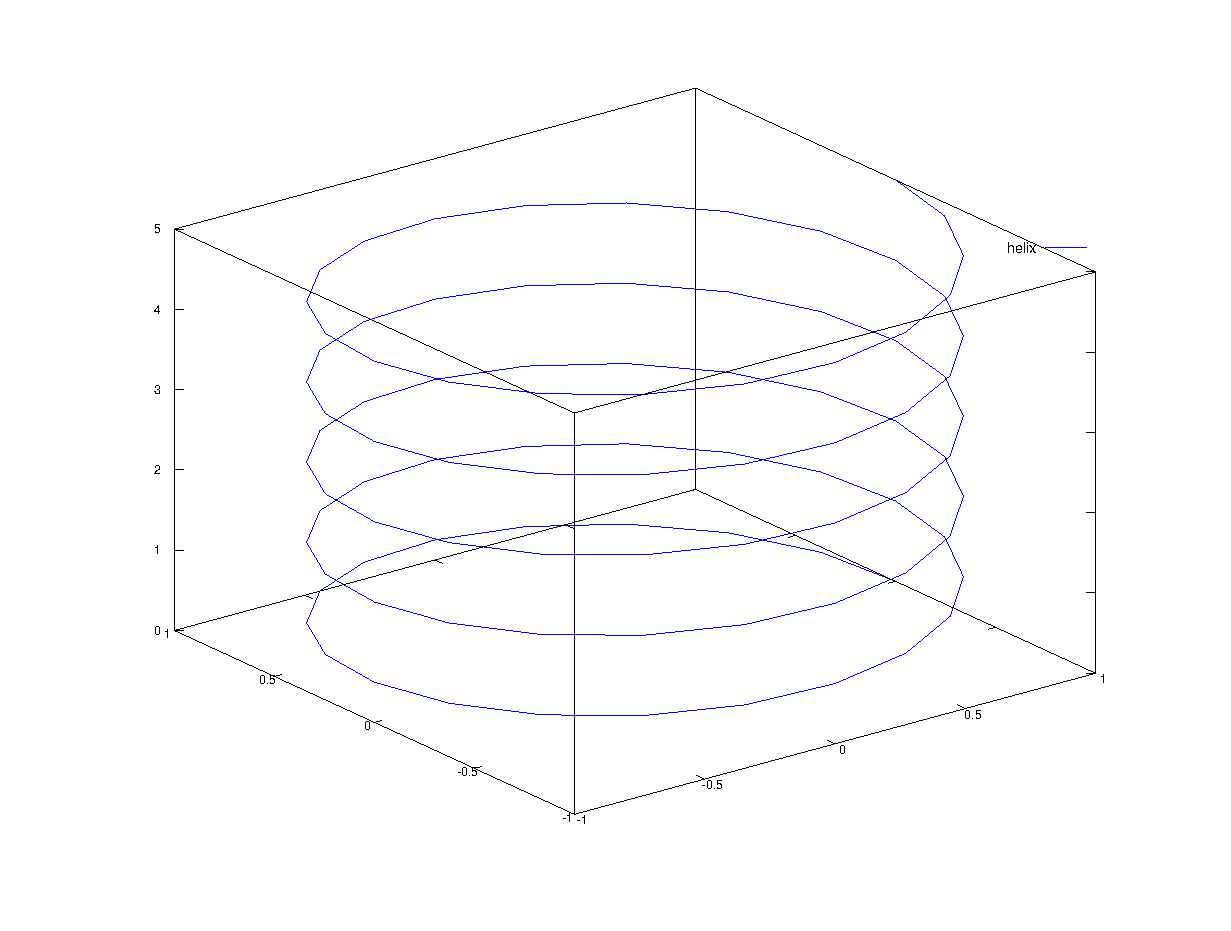
\includegraphics[width=0.6\textwidth]{plot3.eps}
 \caption{{\tt plot3}命令实例——螺旋线}
 \label{plot3}
\end{figure}
\subsection{调整视角}
如果你想改变3D绘图结果的视角,最简单的方法就是使用鼠标(使用鼠标点击并拖拽可以旋转图像,具体
操作选项见表~\ref{tab:view}~)。而Octave的{\tt view}命令能够定量的确定一个特定的视角
(使用{\tt help view}获得更多帮助信息)。
\begin{table}
 \centering
 \begin{tabular}{|l|l|}
 \hline
 鼠标动作 & 操作 \\
 \hline
 LMB+motion & 旋转视角 \\
 <Ctrl>+LMB+motion & 旋转坐标轴(Rotate axes\footnote{不知道和第一个操作有何区别}) \\
 \hline
 快捷键 & 操作 \\
 \hline
 $\rightarrow$ & 右旋 \\
 $\uparrow$    & 上旋\\
 $\leftarrow$  & 左旋\\
 $\downarrow$  & 下旋\\
 \hline
 \end{tabular}
 \caption{切换视角操作}
 \label{tab:view}
\end{table}

另一种重要的的3D绘图便是曲面的绘制。定义一个二元函数$f(x,y)$,该函数的曲面可以用
一系列的Octave的工具画出。首先,要初始化一个网格点,用{\tt meshgird}命令实现:
\begin{verbatim}
 octave:17> x=2:0.2:4;
 octave:18> y=1:0.2:3;
 octave:19> [X,Y]=meshgrid(x,y);% make the grid
\end{verbatim}

\subsection{绘制曲面}
二元函数就可以在定义的{\tt X,Y}网格上被定义,例如一个函数
\begin{equation}\nonumber
 f(x,y)=(x-3)^2-(y-2)^2
\end{equation}
定义该函数可以在Octave中输入
\begin{verbatim}
octave:20> Z=(X-3).^2-(Y-2).^2;
octave:21> subplot(2,2,1);surf(Z);title('surf')
octave:22> subplot(2,2,2);mesh(Z);title('mesh')
octave:23> subplot(2,2,3);meshz(Z);title('meshz')
octave:24> subplot(2,2,4);contour(Z);title('contour')
\end{verbatim}
以上命令的结果如图~\ref{surface}~所示。
\begin{figure}
 \centering
 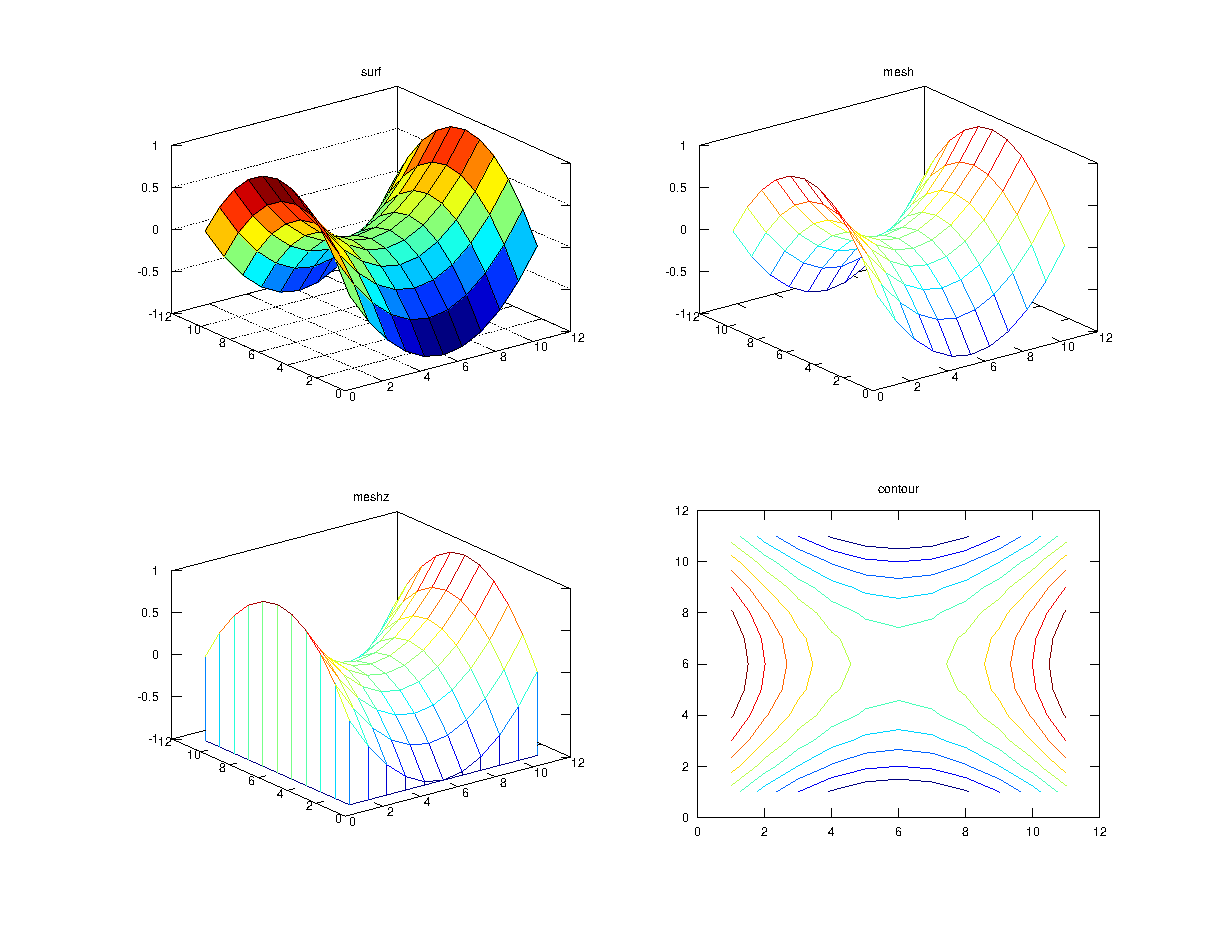
\includegraphics[width=0.6\textwidth]{surface.eps}
 \caption{3D曲面绘制实例}
 \label{surface}
\end{figure}
%section 13
\section{本征向量和奇异值分解}

%section 14
\section{复数}

除了向量和矩阵的计算外,Octave也支持很多在数学或者工程上的概念,比如复数。Octave中
复数的表示法与其常规表达法一致:
\begin{verbatim}
 octave:40> z1=4-3i
 z1 =  4 - 3i
\end{verbatim}
而{\\tt i}和{\\tt j}都可以在Octave中代表单位虚数($\sqrt{-1}$),因此你也可以这样
输入
\begin{verbatim}
 octave:41> z2=1+3j
 z2 =  1 + 3i
\end{verbatim}
普通的复数运算的实例如下:
\begin{verbatim}
 octave:42> z2-z1
 ans = -3 + 6i
 octave:43> z1+z2
 ans =  5
 octave:44> z2/z1 
 ans = -0.20000 + 0.60000i
 octave:45> z1^2
 ans =   7 - 24i
\end{verbatim}
\begin{table}
 \centering
 \begin{tabular}{|lll|}
 \hline
 函数 & 意义 & 表达式 ($z=a+bi$)\\
 \hline 
  {\tt imag} & 虚部 & $a$ \\
  {\tt real} & 实部 & $b$ \\
  {\tt abs}  & 绝对值 & $r=|z|$ \\
  {\tt conj} & 共轭 & $z'=a-bi$ \\
  {\tt angle} & 幅角 & $\theta = \sin(\frac{a}{b})$ \\
 \hline 
 \end{tabular}
 \caption{复数函数}
 \label{tab:comp}
\end{table}
Octave同样的提供了一系列的函数来进行更多的复数计算,比如求复数共轭,模和幅角求解。这些
函数列于表~\ref{tab:comp}~中。而Octave中的内建函数如$\sin(x)$或者$e^x$,都支持
复数。
\subsection{绘制复数}
在Octave下可以用{\\tt plot}命令来创建Argand图(其中$x$轴代表实部而$y$轴代表虚部):
\begin{verbatim}
 octave:3> plot(z1,'*',z2,'*')
 octave:4> axis([-5 5 -5 5])
\end{verbatim}
该命令的结果如图~\ref{complex}~所示。
\begin{figure}
 \centering
 \includegraphics[width=0.6\textwidth]{complex.eps}
 \caption{绘制复数}
 \label{complex}
\end{figure}
\subsection{多项式求根}
Octave提供了一个名为{\tt roots}的命令来求解多项式的根。方程通过其系数的向量表示出来
传递给{\\tt root}函数,例如
\begin{equation}\nonumber
 x^5+2x^4-5x^3+x+3=0
\end{equation}
将被表示为
\begin{verbatim}
 octave:##> c=[1 2 -5 0 1 3];
\end{verbatim}
而{\\tt roots}函数通过以下方式调用
\begin{verbatim}
 octave:12> roots([1 2 -5 0 1 3])
 ans =

  -3.44726 + 0.00000i
   1.17303 + 0.39021i
   1.17303 - 0.39021i
  -0.44940 + 0.60621i
  -0.44940 - 0.60621i
\end{verbatim}
\section{Octave可执行程序}
通过使用类Unix系统中的脚本机制,你可以创建一个Octave可执行程序.通过使用这样的
可执行程序你可以在不用了解程序内容的情况下直接在系统中调用它,这样的程序在批处理
数据文件的时候同样非常有用.一旦一个算法在Octave的交互式终端中被验证为有效的,你就
可以将它写成一个可执行程序并反复对新的数据文件使用.

举一个简单的实例,你创建一个包括如下内容的名为{\tt hello}的文本文件:
\begin{verbatim}
     #!octave-interpreter-name -qf
     # a sample Octave program
     printf ("Hello, world!\n");
\end{verbatim} 
(其中octave-interpreter-name是系统中Octave的绝对路径下的可执行程序名称, 如/usr/bin/octave).
而且该文件的第一行必须以`\verb+#!+'开头.通过为该hello文件添加可执行权限(e.g. chmod u+x hello),
你就可以在系统的终端中输入
\begin{verbatim}
 hello
\end{verbatim}
来执行该文件.
`\verb+#!+'那一行将列出用于解释文件中语句的解释器的绝对路径和名称,而且还可以为该解释器指定一定的
执行选项. 该行中紧接着`\verb+#!+'字符的便是Octave这个程序的路径.而余下的选项便是执行Octave解释器
时的一些参数,例如上面的`-qf'选项中,`-q'选项能够屏蔽程序在普通情况下执行时输出到标准输出的一些介绍
性的信息,而`f'选项能够让程序忽略用户的在文件\verb+~/.octaverc+中的一些设置\footnote{比如,如果
你的Octave程序中调用了一些自定义的函数,而这样的函数在你自定义的path中,那么使用`-f'选项时,Octave
会报错表示无法找到你的那个特定的函数.}.

Octave程序在系统终端执行的时候,还可以为其添加一些参数.这样的参数通过Octave的内部变量{\tt argv}
存储.例如一个例子:
\begin{verbatim}
  #! /bin/octave -qf
     printf ("%s\n", program_name ());
     arg_list = argv ();
     for i = 1:nargin
       printf (" %s\n", arg_list{i});
     endfor
     printf ("\n");
\end{verbatim}
将上述内容保存为test文件中,并为其添加可执行权限并执行之:
\begin{verbatim}
 kasion@tmp:$ chmod u+x test
 kasion@tmp:$ ./test arg1 arg2 arg3
\end{verbatim}
那么程序的输出为:
\begin{verbatim}
 kasion@tmp:$ ./test arg1 arg2 arg3
 test
 arg1
 arg2
 arg3
\end{verbatim}
如果将test文件加入到系统PATH变量所在的目录中(比如/usr/bin或者/home/kasion/bin下),那么
你就可以像调用ls,cd等命令一样调用test命令了,而且通过与系统shell script的灵活调用,能够实现
强大的功能.

最后我给出一个我学习中的一个实际例子,我需要计算一个数据文件中的数据并得到一些图片.
\begin{verbatim}
 1.3000000000e+00 2.9549292750e+00 2.9349509600e+00 
 1.3102040816e+00 2.9454196710e+00 2.9248815610e+00 
 1.3204081633e+00 2.9359134520e+00 2.9148026660e+00 
 1.3306122449e+00 2.9264083650e+00 2.9047117190e+00 

...
\end{verbatim}
其中文件的第一行为波长数据,第二行和第三行为对应波长下波导TE和TM模式的有效折射率数据.
我要求的是其色散系数
\begin{equation}
 D=-\frac{\lambda}{C}\frac{{\rm d}^2 n_{eff}}{{\rm d}\lambda ^2}
\end{equation}
我命名一个Getdistetm的脚本:
\begin{verbatim}
!/usr/bin/octave -q
# no comments...
#print the messages
clear all;
printf("Programe name :%s\n", program_name ());
printf("Processing ....\n");
format long;
#basic constants
C=3e2; # light speed in freespace [um/ps]  
#load the data
arglist=argv ();
...
#load the data
buffer=load(arglist{1});
lam=buffer(:,1);
neffte=buffer(:,2);
nefftm=buffer(:,3);

#caculate the dipersion
fitorder=4;
Pte=polyfit(lam,neffte,fitorder);
Ptm=polyfit(lam,nefftm,fitorder);
for k=1:(fitorder-1)
	P2te(k)=(fitorder+1-k)*(fitorder-k)*Pte(k);
	P2tm(k)=(fitorder+1-k)*(fitorder-k)*Ptm(k);
	end
d2neffte=polyval(P2te,lam);
....
outdata=[lam Dispersionte Dispersiontm];

#save the result 
save("-ascii",outfile,"outdata");
#plot and save the figure;
figure;
plot(lam,Dispersionte,'k:','LineWidth',2,lam,Dispersiontm,'r-','LineWidth',2);
...
grid on;
print(figurename,'-dpng','-S680,500');
printf("Done!\n");
# End of the script
\end{verbatim}
那么执行该脚本的方法为
\begin{verbatim}
 kasion@tmp:$ Getdistetm 800x500_bp_mode_neffr.dat
\end{verbatim}
我将在工作目录下得到该文件对应结构的色散数据和图像.而且通过shell的强大功能,如
\begin{verbatim}
 kasion@tmp:$ for file in `ls *neffr.dat`; do Getdistetm $file; done
\end{verbatim}
就能够将当前目录下所有以neffr.dat结尾的数据执行求色散工作.
\appendix
\section{更多参考资料}
通过以下资料了解更多:
\begin{itemize}
\tiem Octave官方文档:\href{http://www.gnu.org/software/octave/docs.html}{http://www.gnu.org/software/octave/docs.html}\\
\item Octave快速指南:\href{http://ljk.imag.fr/membres/Christophe.Prudhomme/courses/octave/octave-refcard-a4.pdf}{http://ljk.imag.fr/membres/Christophe.Prudhomme/courses/octave/octave-refcard-a4.pdf}\\
\item Octave邮件列表:\href{http://octave.1599824.n4.nabble.com/}{http://octave.1599824.n4.nabble.com/}\\
\end{itemize}

\section{声明}
本文是Dr.P.J.G Long所著的<Introduction to Octave>的部分翻译稿,原文的Acknowledgements如下:\\
\begin{quotation}
 This document has been produced as a tutoial to acompany the version of Octave supplied on the Cambidge-MIT
Institute(CMI)\footnote{CMI-www.cambridge-mint.org} funded Multidisciplinary Design Project (MDP)\footnote{MDP-http://www-mdp.eng.cam.ac.uk}
Resource CD.

The text of this tutorial has been adapted from the student notes developed by Dr. Paul Smith from the 
Cambridge University Engineering Department for a 2nd year Introduction to Matlab sourse. Conversion 
from Paul Smith's original to this current document has be relative easy with in many cases needing only
to exchange
\begin{itemize}
 \item Octave for Matlab in the text
 \item the prompt and precise format of the answers given in the example scripts
 \item removal of specific course administration.
\end{itemize}
However in number of cases there are significant differences, e.g. graphical performance (Gnuplot is 
assumed to be the output plugin for Octave), where changes have had to be made.

Any success of this tutorial is a major result of the the backgroud work carried out by Tim Froggatt in 
setting up the MDP resource distribution and requests from Gareth Wilson,  the author of the RED Tools 
web interface for Octave scipts, for additional information and scripts.

Significaant reference has been made to the resources generated and maintianed by John Eaton and his team at 
www.octave.org. As indicated above, the tutorial is heavily based on Paul Smith's Original in which he 
acknowledges advice and help from Roberto Cipolla, Richard Prager, Hugh Hunt, Maurice Ringer, David Mansergh
and Martin Szummer.
\end{quotation} 
\newpage
本文是我在2011年寒假期间陆续做出来的。随着本工作的展开,我越来越是怀疑本工作的必要性:因为我认为任何有一定的Matlab基础的人
是很容易上手Octave。所以这个工作陆续做下来之后我不免偷工减料,比如原文中的部分小节和章节并没有出现在本译稿中。另外,我
在文中添加了<Octave可执行程序>一节,Octave的这个功能对于我的日常数值计算有很大的帮助。对于文中很多的
不通顺的中文,我在这里向大家表示歉意。而除了不通顺的中文外,文中的\LaTeX{}排版方面也有很多的不足,我的kile程序在编译的时候会
给出大量的error信息。原文中可能有的错误我也没有过多的核查,对于这样的错误我在译稿中姑且是以讹传讹,在这里也希望大家能够积极指
出来。总之,看到这份文稿的你对于该文档有任何的意见和建议都可以通过邮件与我取得联系:\\
联系我:\href{mailto:liuqiang@coer.zju.edu.cn}{liuqiang@coer.zju.edu.cn}

感谢父母在寒假期间对我生活上的无微不至的照顾,让我有时间在电脑前码字。
\end{document}
